\section{Name Management}
The name management layer addresses point \ref{nw} in section~\ref{sec:shortcomings}.  It provides a high-level
narrow waist for access sensors in context specified in the name itself.
StreamFS manages two namespaces.  The first is a flat namespaces that identifies a particular
object instance.  The second is a hierarchical namespace that identifies the current instance
of a particular object in some context, specified by the path for the object.  
We support two namespaces in order to uniquely identify sensors and actuators while supporting multiple names.

Supporting multiple names for points in the building is requirement in applications.  Sensors and actuators can be accessed in various 
ways, depending on the application.  Some applications access the sensors in the context of its placement 
in space.  For example, in Soda Hall, the path \texttt{/soda/4F/410/temp} refers to a temperature sensor in room 410.  
The same temperature sensor drives the fans and heating/cooling sub-system in the HVAC system that serves room.
Other applications refer to this sensor through its association to that sub-system.  For example,
\texttt{/soda/hvac/ahu1/temp} gives that contextual information in the name by using a path name that refers to the the specific
air-handling unit in the HVAC system that the temperature sensor drives.
In the rest of this section we discuss how both namespaces are managed and implemented.

\subsection{Object identifier namespace}

When a new object that is created it is assigned a 128-bit unique identifier that uniquely identifier. % the object.
This flat namespace is large enough to support to many objects with low probability of collisions, even across
StreamFS instances.
% Because StreamFS supports multiple names that refer to the same object, we create a namespace that is 
% flat and large enough to uniquely identify objects in the building uniquely.  
% The unique identifier
% is randomly constructed and the probability of collisions is small because of the large namespace.
StreamFS only assigns a unique identifier to stream and control files, since these represent unique channels for a specific 
object in the deployment.  We discuss StreamFS file types in section~\ref{chap:naming}

% \begin{itemize}
% \item 96 high-order bits identify the object
% \item 32 low-order bits identify the version of the object
% \end{itemize}

% In this paper we concentrate on the high-order bits used to identify the object.  Management of the low-order
% bits is the subject of related, ongoing work.

\subsection{Hierarchical Namespace}

Hierarchical naming schemes are an effective way to organize information, particularly for a relatively small amount of information
where the access patterns are well defined and groups across buildings have a lot of overlap.  For example, upon close examination of
the naming scheme for points across Sutardja Dai Hall, Soda Hall, Cory Hall, and the University of Tokyo Engineering Building 2, we 
observe that there are 2 overlapping group types.  All the point name refer to the location of the sensor and the system that it is 
associated with.  For example, `SODA1R430A\_ART' encodes the name of the building and the room number but also encodes the HVAC subsystem id --
referred to by the 5th character which is a `1'.  The other common encoding include the type of sensor and implies the S.I. units of measure.
Based on our experience with anlysis jobs on building sensor data, we decide it was less import from a naming persepctive than 
an interpretive one.

Because of the number of sensors in the building is on the order of one to ten thousand we adopt the principles articulated 
in~\cite{hierarchy_is_dead}, which asserts that hierarchical organization of files is ineffective when dealing with a large number of files
and that databases are poor at providing direct access to the data, but provide a good way to find the information we are looking for.
We combine these two, as suggested by the authors.  We expose a hierarchical namespace that gives the user direct access to the data
through a familiar organization of that data.  The organization itself is directly traversable.  Moreover, we separate the metadata from
the naming structure, so that users looking for various kinds of information can quickly locate it.

The decision to separate these also gives our implementation \emph{better scalability}.  The growth of the namespace, metadata, and data
happen at different rates.  For example, files and often added and removed, but after creation, changes to the metadata occur less
often that writes to stream file (data produced by sensors).  Moreover, since the 3 kinds of meta/data are accessed in different ways,
we tailor its acquisition to the information being fetched and separate how where/how we store each. % depending on the type of information
%being requested.  
For example, if the query is metadata-related, we send it to the metadata management cluster, which not only stores
the metadata, but also indexes it accordingly.  The data is stored in a time-series database, and the namespaces are stored in a relational
database.  This allows each to grow separately and maximizes fetch efficiency.  Overall, the hierarchical namespaces provides 
\emph{extensibility and ease of management}.
% Because the hierarchical namespace is easily extendable, it provides a natural
% way to group items which eases \emph{management and access}.
We discuss our naming structure in more detail in Chapter~\ref{chap:naming} and give an overview of fundamental challenges that emerge when
naming must reflect physical associations and the physical environment is changing.

\subsection{Implementation Details}

The name management layer is implemented behind HAProxy, an open source load balancer. The implementation includes 
a name registry and a name server.  Several name server handles requests that are forwarded
from HAPRoxy to one of the name servers.  Each of the name server knows of each of the databases that contains names. 
In all our deployments, we only had a single server.  However, for deployments that are large, we put the names in multiple, 
replicated databases with a write-through update policy.  Reads are done from any of the database servers, randomly, since
they all contain the same information.  %Each name server has a preference, so the load is properly distributed.

\begin{figure}[h!] %htbp
\centering
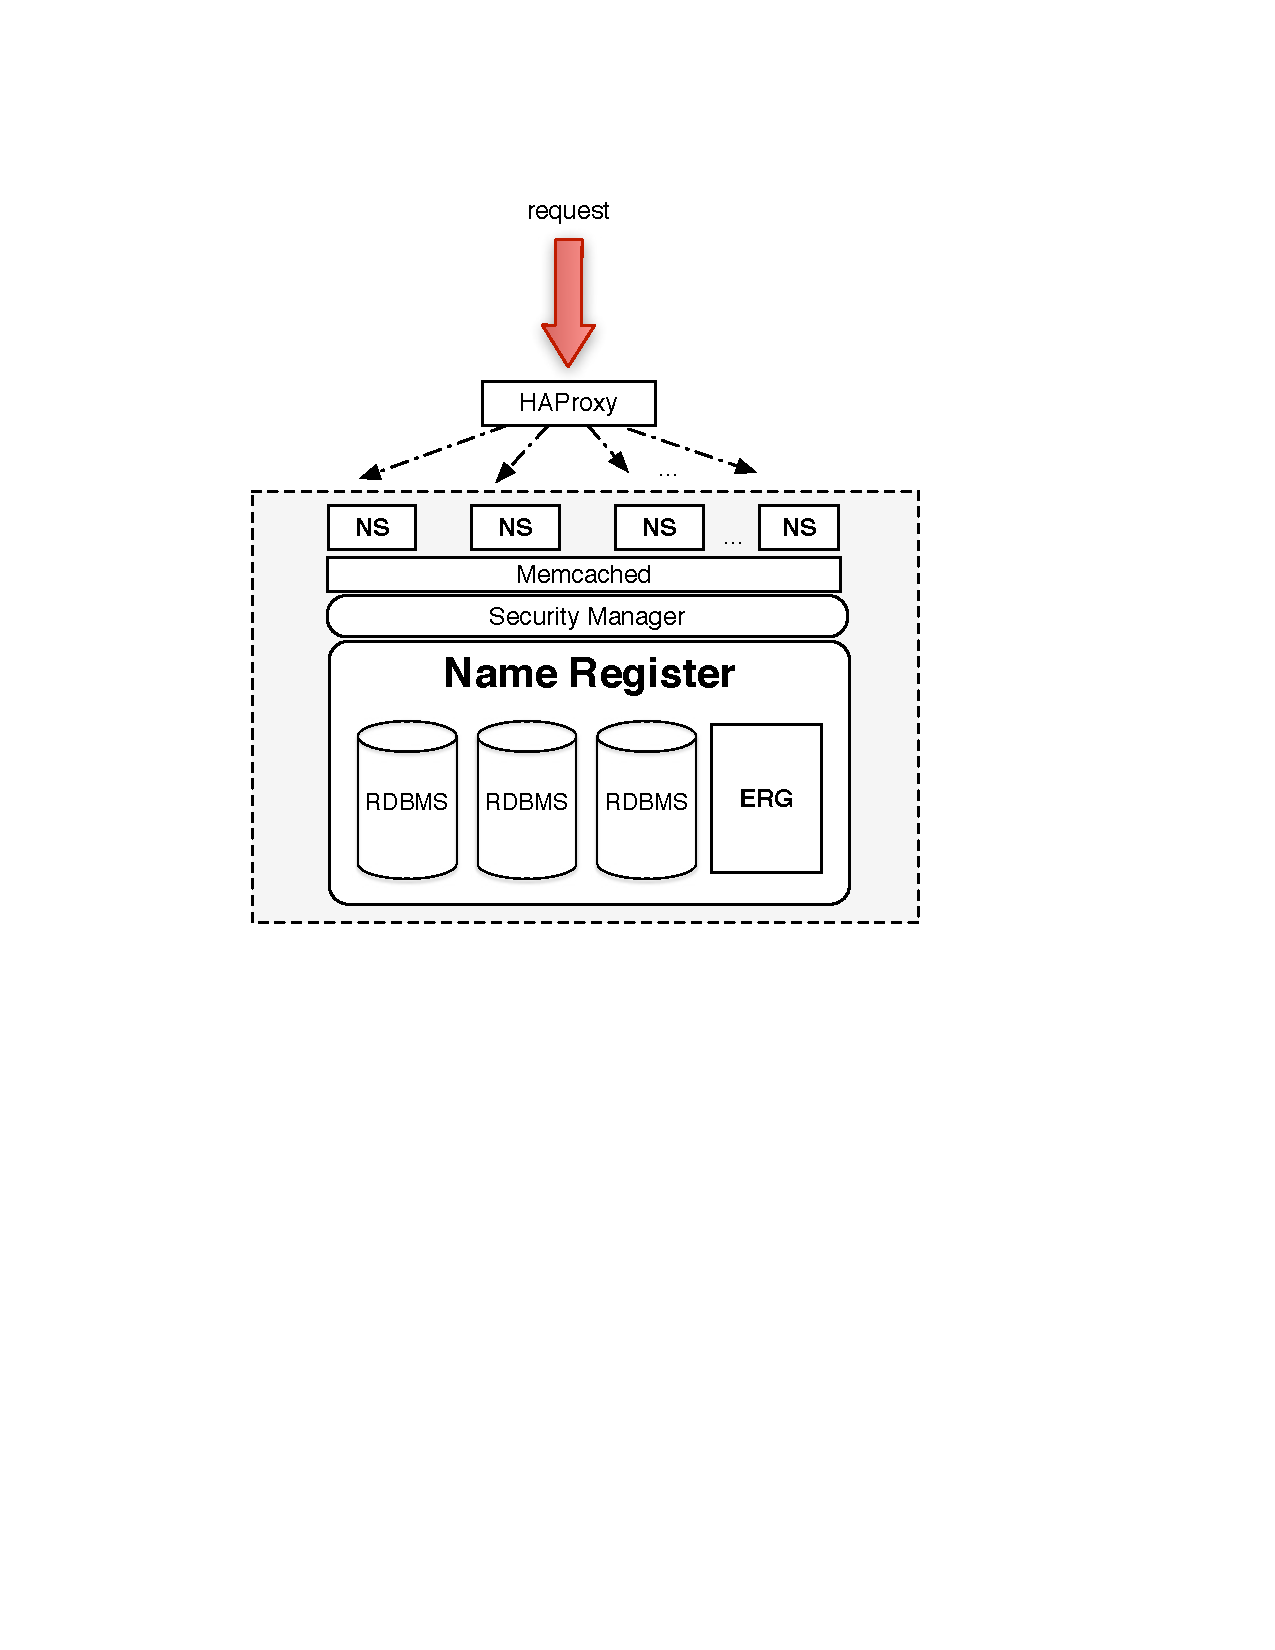
\includegraphics[width=.55\columnwidth]{figs/name_reg}
\caption{Name management layer implemented behind HAProxy.  Name servers handle individual requests and use the name registration table
query handle the request accordingly.}
\label{fig:nameserver}
\end{figure}

The write-through policy is implemented with a write lock.  Whenever a name server receives a request to create or delete a file it informs the
other name servers that it wishes to acquire a lock.  To prevent deadlock, we force a lock-acquisition order.  A lock is not acquired unless every
name server agrees to give up the lock to the requesting name server.  Once the lock is acquired, the name server performs the same write on each
server.  The name server then releases the lock by contacting the other name servers in reverse order.  If a name server has given up a lock
and not received a release, the lock is released automatically after some time.  If a name server goes down, the name server that acquired the lock
assumes the release was successful.  The name server list is immutable, they are restarted in practice if they go down.

A layer of memcached~\cite{memcached} is used to reduce the load on the databases.  Writes immediately invalidate any entries in memcached.  
We also include file metadata in the memcached layer, so its use reduces the load on both the name register and the metadata store.
The security manager essentially maintains an access control list and set of operations that are supported by each file.  By default, 
security is disabled, but some of our deployments do enable it.

The name management layer consists of 3 dependent components, each following the principles of horizontal \emph{scalability}.  The namespaces are
managed in single replicatable, relational database.  The metadata is managed in a separate MongoDB~\cite{mongodb} database, which is itself
shardable.  The data associated with streams is managed in a timeseries database.  We follow the principle of scale-out
in each sub-component, for \emph{scalability}.











